\documentclass[a4paper,12pt]{article}

%% Language and font encodings
\usepackage[portuguese]{babel}
\usepackage[utf8x]{inputenc}
\usepackage[T1]{fontenc}

%% Sets page size and margins
\usepackage[a4paper,top=3cm,bottom=2cm,left=3cm,right=3cm,marginparwidth=1.75cm]{geometry}

%% Useful packages
\usepackage{amsmath}
\usepackage{graphicx}
\usepackage[colorinlistoftodos]{todonotes}
\usepackage[colorlinks=true, allcolors=blue]{hyperref}
\usepackage{listings}
\usepackage{float}
\usepackage{hyphenat}
\usepackage{inconsolata}

\usepackage{color}
\usepackage{fancyhdr}
\pagestyle{fancy}
\lhead{Universidade do Minho - Departamento de Informática}
\rhead{}

\setlength{\headheight}{13.6pt}

\definecolor{pblue}{rgb}{0.13,0.13,1}
\definecolor{pgreen}{rgb}{0,0.5,0}
\definecolor{pred}{rgb}{0.9,0,0}
\definecolor{pgrey}{rgb}{0.46,0.45,0.48}

\usepackage{listings}
\lstset{language=Java,
  showspaces=false,
  showtabs=false,
  breaklines=true,
  showstringspaces=false,
  breakatwhitespace=true,
  commentstyle=\color{pgreen},
  keywordstyle=\color{pblue},
  stringstyle=\color{pred},
  basicstyle=\ttfamily
}

\title{Sistema de negociação}
\author{Hugo Abreu | A76203 \and João Padrão | A76438\and João Reis | A75372
\\\\ Paradigmas de Sistemas Distribuídos \\ \textbf{Universidade do Minho} \\ \\ 
\includegraphics[scale=0.25]{um_eeng}}


\begin{document}

\maketitle


\section{Introdução}
O seguinte trabalho prático advém da necessidade de aplicação e consequente cimentação de conhecimentos adquiridos nas aulas relativas à unidade curricular de Paradigmas de Sistemas Distribuídos, visando temas como a correcta implementação de protocolos de comunicação inter-linguagens e compreenção das temáticas associadas. Assim sendo, o presente relatório reporta à fase final do projeto, estando, por conseguinte, visada a correta implementação de \textit{Protocol Buffers}, tanto em Java com em Erlang. Nesta fase final é também esperado que os conhecimentos acerca de atores, implementação de abordagens com recurso a Message Oriented Middleware e serviços REST sejam corretamente aplicados. 
\par Estratégias para a manipulação das tecnologias contempladas pela Exchange terão de ser adotadas. No final deste projeto, espera-se que tenham sido corretamente aplicados conceitos com significativa complexidade no âmbito da disciplina, de um modo organizado e estruturado, a fim de lançar as fundações adequadas à execução deste último segmento da componente prática de avaliação da unidade curricular.

\section{Front-end Server}

\section{Exchange Server}

\par De modo a processar ordens recebidas, foi necessário implementar um servidor que efetua transações para um para um dado mercado - \textit{PSI20}, \textit{NADAQ}, etc – o que implica que existirá várias instancias deste tipo de servidor a executar. Caberá, portanto, ao \textit{front-server}, assim que recebe uma ordem, averiguar qual o mercado onde uma empresa se encontra e redirecionar para o servidor correto. 

\par Para iniciar um servidor \textit{Exchange}, é necessário indicar sobre parâmetro qual o mercado onde irá operar de modo a obter as informações necessárias via REST. Dada cada empresa recebida, é criado um objeto \textit{Company} que conterá queues de ordens de compra e venda, que não foram de imediato efetuadas uma transação. Está associado também um objeto \textit{PriceInfo}, que contem os preços de abertura, fecho, máximo e mínimo. Sempre que uma transação é efetuada, este verifica com os valores contidos se existem alterações, e se conferir, é enviado ao servidor REST.

\par Este conjunto de objectos encontram-se agregados num mapa que será acedido por todas as conexões. 

\par Entre essas informações obtidas, encontra-se também a porta onde irá escutar novas conexões do provenientes do \textit{front-server}. É também iniciado um \textit{Publisher} implementado em ZeroMQ, que publica informação sempre que uma transação é efetuada.

\par Estando, portanto, à escuta de novas conexões, estas originam um novo \textit{Handler} que recebe um \textit{protobuff order}. Se hora de receção estiver entre as 9:00 e 17:00 é replicado o \textit{protobuff} recebido, indicando desta vez uma confirmação positiva e enviado para o socket, processando o pedido posteriormente. Caso contrário, envia-se apendas uma confirmação negativa.

\begin{figure}[h]
  \centering
      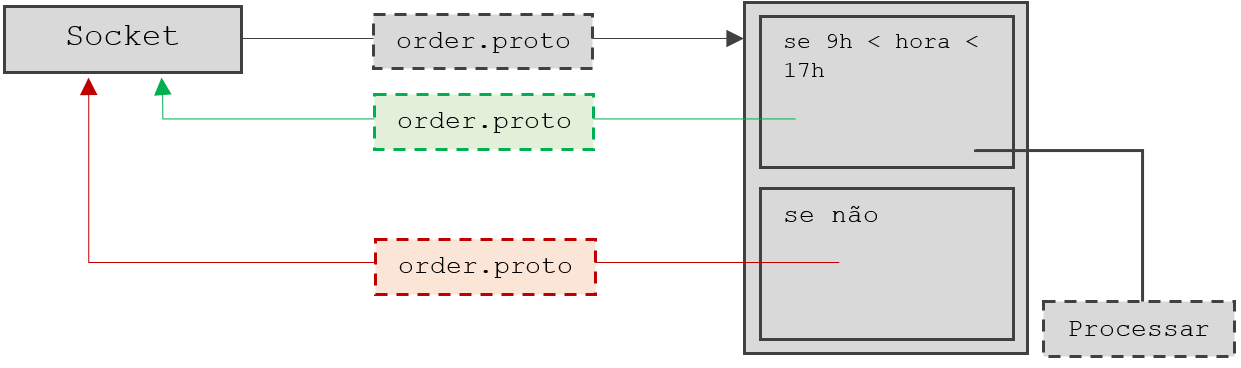
\includegraphics[width=1\textwidth]{d1.PNG}
  \caption{Aceitação de conexões}
\end{figure}

\par A \textit{protobuff} order recebida é encaminhada para o objeto correspondente à empresa a que diz respeito. Consoante o tipo de order – compra ou venda – confere-se na contrária queue se existem outras que correspondam de modo a efetuar uma transação. No fim, se ainda existir quantidade por vender, é também colocada em queue.
\par Sempre que uma transação é efetuada, são enviados a ambos intervenientes (via \textit{front-server}, que estará à escuta na porta 3001) uma confirmação usando novamente uma protobuff order com a quantidade transacionada, assim como o preço a que foi feita.  É também enviado ao publisher uma mensagem para anunciar a transação entre os dois utilizadores, bem como a quantidade e o preço.  


**FALAR DO TIMER PARA O CLOSE**

\section{Directory Server}
Para projetar o servidor de directório, ou seja, o servidor que contém todos os meta-dados relativos ao sistema de negociação, portanto, esta entidade do sistema mantém dados como, que empreas existem, em que exchange são transacionadas, que exchanges existem e que empresas têm e, os diferentes preços diários das empresas em questão. A utilização de um servidor REST para este tipo de acesso a dados, é o mais correto, visto que não existe a necessidade de manter estado entre pedidos e, desta forma, faz com que um só servidor consiga suportar muitos utilizadores em simultâneo.
\par O servidor construído, tal como requirido pelo docente no enunciado, é um servidor REST, stateless, programado em Java com recuros a framework Dropwizard. Para ser possível garantir o acesso a todos os recursos que o serviço oferece, foi necessário definir \textit{end-points} para obter e/ou atualizar esses mesmos recursos. Os \textit{end-points} definidos para o servidor REST foram os seguintes:

\begin{itemize}
\item GET
  \begin{itemize}
    \item \textbf{/companies}
    \par Este \textit{end-point} devolve uma lista com todas as empresas existentes no sistema. A lista devolvida é uma lista de objetos e, portanto, contém todos os atributos intrínsecos a cada empresa na enumeração.
    
    \item \textbf{/company/{id}}
    \par Este recurso, quando fornecido um correcto id de empresa, a respetiva empresa, caso esta se encontre efetivamente no sistema. Neste recuso é devolvida a empresa e todos os atributos a esta relacionados.
    
    \item \textbf{/company/{id}/today}
    \par O \textit{end-point} descrito neste ponto, devolve a informação de preços do dia corrente, sendo que, esta informação também é devolvida no recurso anterior, desta forma, caso apenas seja necessário obter os preços, é possível reduzir a quantidade de informação que circula na rede.
    
    \item \textbf{/company/{id}/yesterday}
    \par Da mesma forma que o recurso mencionado anteriormente retorna os preços do dia atual, este recurso retorna os preços do dia anterior.
    
    \item \textbf{/exchanges}
    \par Este \textit{end-point} devolve uma lista com todas as exchanges existentes no sistema. A lista devolvida é, tal como nas empresas, uma lista de objetos e, portanto, contém todos os atributos intrínsecos a cada exchange na enumeração.

    \item \textbf{/exchange/{id}}
    \par Quando o recurso descrito é acedido, ao fornecer um id de exchange válido, este recurso devolve a dita exchange com todos os astributos a ela relacionados, como por exemplo, o IP+Porta.

    \item \textbf{/exchange/{id}/companies}
    \par Este \textit{end-point} devolve uma lista com todas as empresas da exchange que é fornecida como argumento (id). A lista devolvida é uma lista de objetos e, portanto, contém todos os atributos intrínsecos a cada empresa.
    
    
  \end{itemize}
\item PUT
  \par Os recursos definidos como PUT, deverão ser idempotentes, ou seja, por muitas vezes que o recurso seja executado, o resultado é o mesmo e, portanto, é a operação ideal para, neste caso, o recurso listado abaixo.
  \begin{itemize}
    \item \textbf{/company/{id}/today}

    \par Este recurso tem como objetivo atualizar os preços atuais de uma dada empresa e, portanto é uma operação idempotente visto que, o resultado é sempre o mesmo não importando a quantidade de vezes que é executado.
  \end{itemize}
\end{itemize}

\par Todos os recursos abordados acima foram corretamente implementados e a sua executção foi efetivamente testada, o grupo teve o cuidado de utilizar as primitivas da framework Jackson para permitir a correcta serialização dos dados.
\par Foi também adicionada a funcionalidade ao REST server de às 23:59:59 de cada dia, executar a alteração diária, ou seja, às horas definidas, é accionado um \textit{trigger} que vai a todas as empresas trocar os preços actuais para o dia anterior, garantindo assim a atualização das informações no directório.

\section{Client}
Para permitir o acesso às funcionalidades completas da Exchange e todos os recursos do eco-sistema associado, foi construído um Client que visa a utilização por utilizadores ditos normais.
\par No cliente foram aplicadas todas as funcionalidades requiridas pelo docente no enunciado disponibilizado, as opções de um utilizador com o login efetuado são as seguintes:
\begin{verbatim}
[1] Ver empresas.
[2] Ver exchanges.
[3] Ver uma empresa específica.
[4] Verificar preços da empresa.
[5] Obter real time updates.
[6] Cancelar real time updates.
[7] Abrir posição.
\end{verbatim}
\par As operações descritas são operações que, além de requiridas no enunciado do trabalho prático, são necessárias para a correta funcionalidade de toda a aplicação. A opção \textbf{[1]}, contacta o serviço de directório (REST) de forma a obter a lista de todas as empresas que se encontram disponíveis para transacionar, 

\section{Conclusão}
Com o término da fase final do projeto, é admissível afirmar que todos os objetivos requeridos pelo docente no enunciado cedido foram alcançados.
\par Conhecimentos relativos à implementação de Message Oriented Middleware, serviços REST, Protocol Buffers e atores em Erlang foram incrementados e por consequência cimentados. Em relação à linguagem Erlang, o grupo teve a necessidade de utilizar um gerenciador de pacotes semelhante ao Maven, o \textit{rebar3} que, permitiu aprofundar o conhecimento relativo à linguagem e respetiva utilização de diferentes pacotes desenvolvidos nesta.
\par O maior foco incidiu sobre a correta implementação dos diferentes protocolos inter-linguagem e, em particular na implementação do front-end server que é parte fundamental na comunicação de sistemas.
\par A qualidade do trabalho apresentado agrada ao grupo, tendo havido tempo suficiente para o estudo das soluções encontradas ao problema proposto, sem precipitações e com espaço de maneio suficiente para que todos os membros pudessem inteirar-se não somente do segmento que lhes foi atribuído, mas também das restantes duas terças-partes que não exigiram tanta da sua atenção.

\end{document}